\documentclass[11pt,a4paper]{article}

\usepackage[T1]{fontenc}
\usepackage[utf8]{inputenc}
\usepackage[polish]{babel}
\usepackage{lmodern}
\usepackage{amsmath,amssymb}
\usepackage{booktabs}
\usepackage{graphicx}
\usepackage[margin=2.3cm]{geometry}
\usepackage{microtype}
\usepackage{caption}
\usepackage{float}
\usepackage{titlesec}
\usepackage{enumitem}

\captionsetup{skip=3pt}
\titlespacing*{\section}{0pt}{8pt}{2pt}
\titlespacing*{\subsection}{0pt}{4pt}{1pt}
\setlength{\parskip}{3pt}
\setlength{\parindent}{0pt}
\setlist{nosep, leftmargin=14pt}

\title{\vspace{-1.0cm}\textbf{Obliczenia Naukowe - Lista 2}}
\author{Jakub Retmańczyk}
\date{7 listopada 2026}

\begin{document}

\maketitle
\vspace{-0.6cm}

\section{Zadanie 1}

Powtórzyłem zadanie 4 z listy 1 dla danych z usuniętą ostatnią cyfrą: $x_4 = 0.577215664$, $x_5 = 0.301029995$. Wartość dokładną dla nowych danych policzyłem w \texttt{BigFloat}.

\begin{table}[H]
\centering
\small
\caption{Iloczyn skalarny dla danych pierwotnych i zmienionych.}
\begin{tabular}{lcccc}
\toprule
\textbf{Metoda} & \multicolumn{2}{c}{\textbf{Float32}} & \multicolumn{2}{c}{\textbf{Float64}} \\
\cmidrule(lr){2-3} \cmidrule(lr){4-5}
 & pierwotne & zmienione & pierwotne & zmienione \\
\midrule
(a) w przód         & $-0.4999443$ & $-0.4999443$ & $1.025 \cdot 10^{-10}$  & $-4.29634274 \cdot 10^{-3}$ \\
(b) w tył           & $-0.4543457$ & $-0.4543457$ & $-1.564 \cdot 10^{-10}$ & $-4.29634300 \cdot 10^{-3}$ \\
(c) od największych & $-0.5$       & $-0.5$       & $0$                     & $-4.29634284 \cdot 10^{-3}$ \\
(d) od najmniejszych & $-0.5$      & $-0.5$       & $0$                     & $-4.29634284 \cdot 10^{-3}$ \\
\midrule
Wartość dokładna & \multicolumn{2}{c}{} & $-1.007 \cdot 10^{-11}$ & $-4.29634319 \cdot 10^{-3}$ \\
\bottomrule
\end{tabular}
\end{table}

\subsection*{Interpretacja}
\begin{itemize}
    \item Dane zmieniły się względnie o około $2 \cdot 10^{-9}$, a dokładny wynik przeskoczył z $-1.0 \cdot 10^{-11}$ na $-4.3 \cdot 10^{-3}$, czyli o ponad 8 rzędów wielkości. Prawie całą tę zmianę daje składnik $y_4 \Delta x_4$, bo $y_4 \approx 4.8 \cdot 10^{6}$.
    \item Zadanie jest bardzo źle uwarunkowane: dla danych pierwotnych $\sum|x_i y_i| / |\sum x_i y_i| \approx 5.5 \cdot 10^{17}$.
    \item W \texttt{Float64} błąd bezwzględny jest podobny jak wcześniej (rzędu $10^{-10}$), ale wynik jest teraz dużo większy, więc wszystkie metody zgadzają się z wartością dokładną na około 7 cyfrach. Dla danych pierwotnych był to sam szum zaokrągleń, w metodzie (a) nawet ze złym znakiem.
    \item W \texttt{Float32} wyniki w ogóle się nie zmieniły. Po konwersji $x_4$ jest identyczne w obu wersjach, a $x_5$ różni się tylko ostatnim bitem, co ginie przy składnikach rzędu $10^{6}$. Wyniki pozostają błędne: ok. $-0.5$ zamiast $-4.3 \cdot 10^{-3}$.
\end{itemize}


\section{Zadanie 2}

Rozwiązałem $Ax = b$ dla $b = Ax$, $x = (1, \dots, 1)^T$ na dwa sposoby: eliminacją Gaussa (\verb|A\b|) i przez odwrotność (\verb|inv(A)*b|). W tabelach podaję błąd względny $\|\tilde{x} - x\|_2 / \|x\|_2$.

\begin{table}[H]
\centering
\small
\caption{Macierze Hilberta $H_n$.}
\begin{tabular}{rcccc}
\toprule
$n$ & \texttt{cond} & \texttt{rank} & \textbf{Gauss} & \textbf{inv} \\
\midrule
2 & $1.9 \cdot 10^{1}$ & 2 & $5.7 \cdot 10^{-16}$ & $1.1 \cdot 10^{-15}$ \\
4 & $1.6 \cdot 10^{4}$ & 4 & $4.2 \cdot 10^{-13}$ & $4.0 \cdot 10^{-13}$ \\
6 & $1.5 \cdot 10^{7}$ & 6 & $1.5 \cdot 10^{-10}$ & $1.0 \cdot 10^{-10}$ \\
8 & $1.5 \cdot 10^{10}$ & 8 & $3.6 \cdot 10^{-7}$ & $4.0 \cdot 10^{-7}$ \\
10 & $1.6 \cdot 10^{13}$ & 10 & $4.2 \cdot 10^{-4}$ & $4.1 \cdot 10^{-4}$ \\
12 & $1.6 \cdot 10^{16}$ & 11 & $5.5 \cdot 10^{-1}$ & $6.7 \cdot 10^{-1}$ \\
14 & $3.2 \cdot 10^{17}$ & 11 & $9.7$ & $1.0 \cdot 10^{1}$ \\
16 & $2.2 \cdot 10^{18}$ & 12 & $1.0 \cdot 10^{1}$ & $8.4$ \\
18 & $3.3 \cdot 10^{18}$ & 12 & $5.4$ & $3.7$ \\
20 & $6.8 \cdot 10^{18}$ & 13 & $2.9 \cdot 10^{1}$ & $3.1 \cdot 10^{1}$ \\
25 & $3.8 \cdot 10^{20}$ & 13 & $2.4 \cdot 10^{1}$ & $5.2 \cdot 10^{1}$ \\
30 & $2.4 \cdot 10^{18}$ & 14 & $2.6 \cdot 10^{1}$ & $4.3 \cdot 10^{1}$ \\
\bottomrule
\end{tabular}
\end{table}

\begin{table}[H]
\centering
\footnotesize
\setlength{\tabcolsep}{4pt}
\caption{Macierze losowe $R_n$ (jedno losowanie, ziarno 1234).}
\begin{tabular}{rcccccc}
\toprule
 & \multicolumn{2}{c}{$n = 5$} & \multicolumn{2}{c}{$n = 10$} & \multicolumn{2}{c}{$n = 20$} \\
\cmidrule(lr){2-3} \cmidrule(lr){4-5} \cmidrule(lr){6-7}
$c$ & \textbf{Gauss} & \textbf{inv} & \textbf{Gauss} & \textbf{inv} & \textbf{Gauss} & \textbf{inv} \\
\midrule
$1$ & $1.9 \cdot 10^{-16}$ & $1.8 \cdot 10^{-16}$ & $3.9 \cdot 10^{-16}$ & $3.7 \cdot 10^{-16}$ & $5.9 \cdot 10^{-16}$ & $3.6 \cdot 10^{-16}$ \\
$10$ & $1.7 \cdot 10^{-16}$ & $2.6 \cdot 10^{-16}$ & $3.9 \cdot 10^{-16}$ & $2.4 \cdot 10^{-16}$ & $3.3 \cdot 10^{-16}$ & $4.3 \cdot 10^{-16}$ \\
$10^{3}$ & $7.4 \cdot 10^{-15}$ & $7.1 \cdot 10^{-15}$ & $2.9 \cdot 10^{-14}$ & $2.8 \cdot 10^{-14}$ & $3.1 \cdot 10^{-14}$ & $2.6 \cdot 10^{-14}$ \\
$10^{7}$ & $3.5 \cdot 10^{-10}$ & $3.6 \cdot 10^{-10}$ & $7.2 \cdot 10^{-12}$ & $2.8 \cdot 10^{-11}$ & $9.4 \cdot 10^{-11}$ & $1.1 \cdot 10^{-10}$ \\
$10^{12}$ & $2.3 \cdot 10^{-5}$ & $2.5 \cdot 10^{-5}$ & $1.9 \cdot 10^{-5}$ & $1.8 \cdot 10^{-5}$ & $4.6 \cdot 10^{-6}$ & $7.8 \cdot 10^{-6}$ \\
$10^{16}$ & $1.6 \cdot 10^{-1}$ & $1.5 \cdot 10^{-1}$ & $2.2 \cdot 10^{-1}$ & $2.5 \cdot 10^{-1}$ & $1.1 \cdot 10^{-1}$ & $7.7 \cdot 10^{-2}$ \\
\bottomrule
\end{tabular}
\end{table}

\subsection*{Interpretacja}
\begin{itemize}
    \item Dla $R_n$ błąd rośnie razem z $c$, od ok. $10^{-16}$ dla $c = 1$ do ok. $0.1$--$0.2$ dla $c = 10^{16}$, a rozmiar macierzy prawie nie ma znaczenia. Od $c = 10^{3}$ błąd mieści się poniżej $c \cdot \text{macheps}$.
    \item $H_n$ psuje się bardzo szybko: \texttt{cond} rośnie o ok. 3 rzędy na każde dwa stopnie. Dla $n = 10$ zostają 3--4 poprawne cyfry, dla $n = 12$ błąd to już ok. $0.6$, a od $n = 14$ przekracza 1, czyli wynik nie ma nic wspólnego z rozwiązaniem.
    \item $H_n$ jest nieosobliwa, a mimo to od $n = 12$ funkcja \texttt{rank} zwraca mniej niż $n$. Wartościom \texttt{cond} dla $n \ge 14$ też nie można ufać: dla $n = 30$ wyszło mniej niż dla $n = 25$. Podobnie dla $c = 10^{16}$ rząd $R_n$ spadł o 1 (4, 9, 19), a \texttt{cond} wyniosło $7.3 \cdot 10^{15}$, $7.0 \cdot 10^{15}$ i $9.6 \cdot 10^{15}$.
    \item Żadna z metod nie okazała się dokładniejsza: Gauss dał mniejszy błąd w 15 z 30 testów, a błędy są zawsze tego samego rzędu. O wyniku decyduje uwarunkowanie macierzy. W praktyce wybrałbym \verb|A\b|, bo nie trzeba liczyć całej odwrotności.
\end{itemize}


\section{Zadanie 3}

Granica: podstawiając $t = e^{-x}$, mamy $\lim_{x \to \infty} f(x) = \lim_{t \to 0^+} \ln(1 + t)/t = 1$. Wykres narysowałem w Julii (Plots) i w Pythonie (matplotlib). Dla porównania dodałem wersję z \texttt{log1p}, która liczy $\ln(1 + t)$ bez tworzenia sumy $1 + t$.

\begin{figure}[H]
\centering
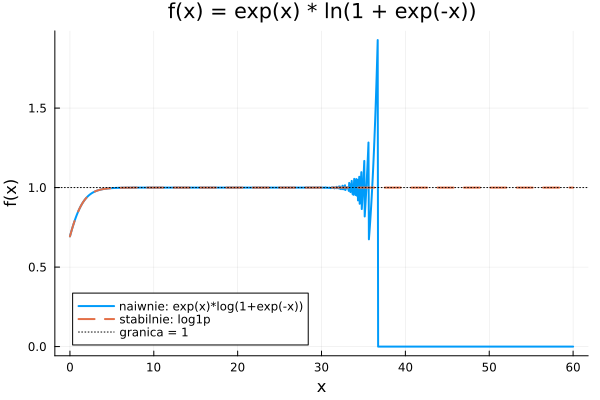
\includegraphics[width=.49\textwidth]{zad3_julia.png}
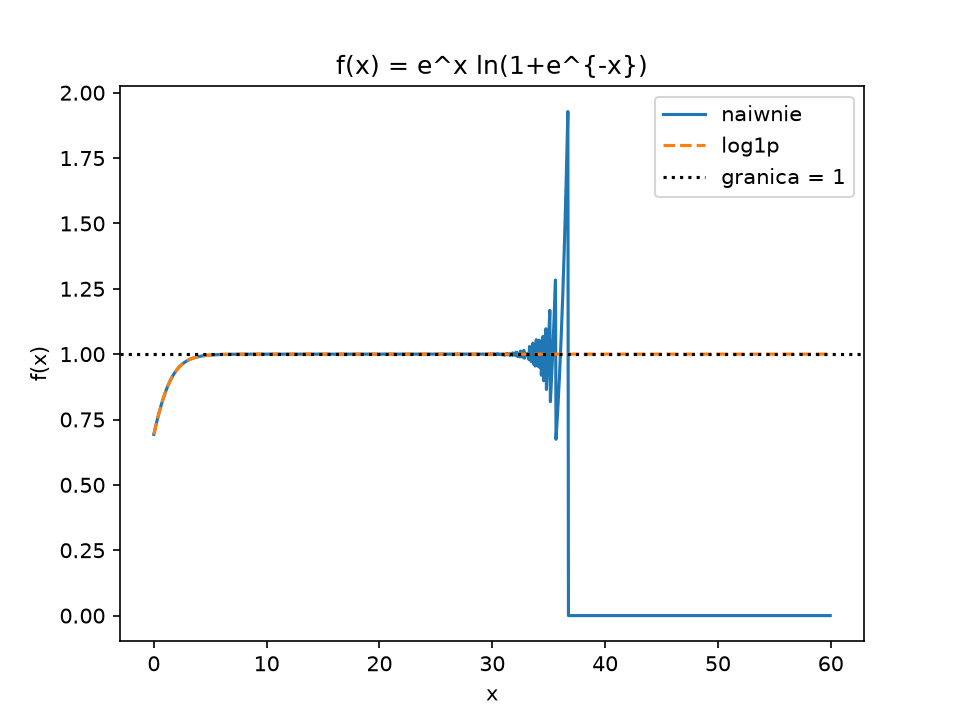
\includegraphics[width=.49\textwidth]{zad3_python.png}
\caption{Wykres $f(x)$ w Julii (po lewej) i w Pythonie (po prawej).}
\end{figure}

\begin{table}[H]
\centering
\footnotesize
\caption{Wartości $f(x)$ w \texttt{Float64}.}
\begin{tabular}{lcccccc}
\toprule
$x$ & $10$ & $20$ & $30$ & $36$ & $36.7$ & $37$ \\
\midrule
wzór z treści & $0.9999773007$ & $1.0000000328$ & $0.9989799652$ & $0.9572857056$ & $1.9277366815$ & $0$ \\
\texttt{log1p} & $0.9999773007$ & $0.9999999990$ & $1.0000000000$ & $1.0000000000$ & $1.0000000000$ & $1.0000000000$ \\
\bottomrule
\end{tabular}
\end{table}

\subsection*{Interpretacja}
\begin{itemize}
    \item Oba programy pokazują to samo. Do ok. $x = 30$ wykres zgadza się z granicą, potem zaczyna oscylować (dla $x$ między $35$ a $36$ w zakresie od $0.67$ do $1.33$), tuż przed $x = 36.74$ dochodzi prawie do $2$, a dalej jest stale równy $0$, choć granica wynosi $1$.
    \item Przy dużym $x$ w sumie $1 + e^{-x}$ zostaje tylko kilka bitów z $e^{-x}$, a mnożenie przez $e^{x}$ wzmacnia ten błąd. Stąd oscylacje. Dla $x \in (35.64, 36.74)$ suma zaokrągla się do $1 + 2^{-52}$, więc $f \approx 2^{-52} e^{x}$ rośnie od $0.67$ do $2$.
    \item Dla $x > 36.74$ mamy $e^{-x} < 2^{-53}$, więc $\text{fl}(1 + e^{-x}) = 1$, $\ln 1 = 0$ i $f = 0$.
    \item Wersja z \texttt{log1p} jest poprawna w całym rysowanym przedziale, więc winny jest sposób liczenia, a nie sama funkcja. Psuje się dopiero przez przepełnienie $e^{x}$: dla $x = 710$ daje \texttt{Inf}, a dla $x = 746$ \texttt{NaN}.
\end{itemize}


\section{Zadanie 4}

Pierwiastki policzyłem funkcją \texttt{roots} z pakietu Polynomials i posortowałem po części rzeczywistej. W przypadku (b) $P$ to wielomian zaburzony, a $p$ nadal oryginalny.

\begin{table}[H]
\centering
\footnotesize
\caption{Sprawdzenie pierwiastków wielomianu Wilkinsona.}
\begin{tabular}{rcccccc}
\toprule
 & \multicolumn{3}{c}{\textbf{(a) współczynniki oryginalne}} & \multicolumn{3}{c}{\textbf{(b) $-210 \to -210 - 2^{-23}$}} \\
\cmidrule(lr){2-4} \cmidrule(lr){5-7}
$k$ & $|P(z_k)|$ & $|p(z_k)|$ & $|z_k - k|$ & $|P(z_k)|$ & $|p(z_k)|$ & $|z_k - k|$ \\
\midrule
1 & $3.6 \cdot 10^{4}$ & $3.7 \cdot 10^{4}$ & $3.0 \cdot 10^{-13}$ & $2.0 \cdot 10^{4}$ & $2.0 \cdot 10^{4}$ & $1.6 \cdot 10^{-13}$ \\
2 & $1.8 \cdot 10^{5}$ & $1.8 \cdot 10^{5}$ & $2.8 \cdot 10^{-11}$ & $3.5 \cdot 10^{5}$ & $3.5 \cdot 10^{5}$ & $5.5 \cdot 10^{-11}$ \\
3 & $2.8 \cdot 10^{5}$ & $2.9 \cdot 10^{5}$ & $4.1 \cdot 10^{-10}$ & $2.3 \cdot 10^{6}$ & $2.4 \cdot 10^{6}$ & $3.4 \cdot 10^{-9}$ \\
4 & $3.0 \cdot 10^{6}$ & $2.0 \cdot 10^{6}$ & $1.6 \cdot 10^{-8}$ & $1.0 \cdot 10^{7}$ & $1.1 \cdot 10^{7}$ & $9.0 \cdot 10^{-8}$ \\
5 & $2.3 \cdot 10^{7}$ & $2.1 \cdot 10^{7}$ & $6.7 \cdot 10^{-7}$ & $3.8 \cdot 10^{7}$ & $4.5 \cdot 10^{7}$ & $1.4 \cdot 10^{-6}$ \\
6 & $1.3 \cdot 10^{8}$ & $1.1 \cdot 10^{8}$ & $1.1 \cdot 10^{-5}$ & $1.3 \cdot 10^{8}$ & $2.1 \cdot 10^{8}$ & $2.1 \cdot 10^{-5}$ \\
7 & $4.8 \cdot 10^{8}$ & $4.6 \cdot 10^{8}$ & $1.0 \cdot 10^{-4}$ & $3.9 \cdot 10^{8}$ & $1.8 \cdot 10^{9}$ & $4.0 \cdot 10^{-4}$ \\
8 & $1.6 \cdot 10^{9}$ & $1.6 \cdot 10^{9}$ & $6.4 \cdot 10^{-4}$ & $1.2 \cdot 10^{9}$ & $1.9 \cdot 10^{10}$ & $7.8 \cdot 10^{-3}$ \\
9 & $4.9 \cdot 10^{9}$ & $4.7 \cdot 10^{9}$ & $2.9 \cdot 10^{-3}$ & $2.2 \cdot 10^{9}$ & $1.4 \cdot 10^{11}$ & $8.4 \cdot 10^{-2}$ \\
10 & $1.4 \cdot 10^{10}$ & $1.3 \cdot 10^{10}$ & $9.6 \cdot 10^{-3}$ & $1.1 \cdot 10^{10}$ & $1.5 \cdot 10^{12}$ & $6.5 \cdot 10^{-1}$ \\
11 & $3.6 \cdot 10^{10}$ & $3.3 \cdot 10^{10}$ & $2.5 \cdot 10^{-2}$ & $1.1 \cdot 10^{10}$ & $1.5 \cdot 10^{12}$ & $1.1$ \\
12 & $7.5 \cdot 10^{10}$ & $7.4 \cdot 10^{10}$ & $4.7 \cdot 10^{-2}$ & $3.1 \cdot 10^{10}$ & $3.3 \cdot 10^{13}$ & $1.7$ \\
13 & $2.0 \cdot 10^{11}$ & $1.8 \cdot 10^{11}$ & $7.4 \cdot 10^{-2}$ & $3.1 \cdot 10^{10}$ & $3.3 \cdot 10^{13}$ & $2.0$ \\
14 & $3.6 \cdot 10^{11}$ & $3.6 \cdot 10^{11}$ & $8.5 \cdot 10^{-2}$ & $2.2 \cdot 10^{11}$ & $9.6 \cdot 10^{14}$ & $2.5$ \\
15 & $8.2 \cdot 10^{11}$ & $8.4 \cdot 10^{11}$ & $7.5 \cdot 10^{-2}$ & $2.2 \cdot 10^{11}$ & $9.6 \cdot 10^{14}$ & $2.7$ \\
16 & $1.6 \cdot 10^{12}$ & $1.6 \cdot 10^{12}$ & $5.4 \cdot 10^{-2}$ & $4.8 \cdot 10^{11}$ & $2.7 \cdot 10^{16}$ & $2.9$ \\
17 & $3.7 \cdot 10^{12}$ & $3.3 \cdot 10^{12}$ & $2.5 \cdot 10^{-2}$ & $4.8 \cdot 10^{11}$ & $2.7 \cdot 10^{16}$ & $2.8$ \\
18 & $7.6 \cdot 10^{12}$ & $6.3 \cdot 10^{12}$ & $9.1 \cdot 10^{-3}$ & $4.6 \cdot 10^{12}$ & $4.2 \cdot 10^{17}$ & $2.5$ \\
19 & $1.1 \cdot 10^{13}$ & $1.2 \cdot 10^{13}$ & $1.9 \cdot 10^{-3}$ & $4.6 \cdot 10^{12}$ & $4.2 \cdot 10^{17}$ & $2.0$ \\
20 & $2.8 \cdot 10^{13}$ & $2.3 \cdot 10^{13}$ & $1.9 \cdot 10^{-4}$ & $8.8 \cdot 10^{12}$ & $1.4 \cdot 10^{18}$ & $8.5 \cdot 10^{-1}$ \\
\bottomrule
\end{tabular}
\end{table}

\subsection*{Interpretacja (a)}
\begin{itemize}
    \item Błąd $|z_k - k|$ rośnie od $3.0 \cdot 10^{-13}$ dla $k = 1$ do $8.5 \cdot 10^{-2}$ dla $k = 14$ i maleje do $1.9 \cdot 10^{-4}$ dla $k = 20$.
    \item Duże wartości $|P(z_k)|$ i $|p(z_k)|$ nie są szumem. Po policzeniu $P(z_k)$ w \texttt{BigFloat} z dokładnymi współczynnikami wychodzi praktycznie to samo co $|p(z_k)|$. Powód: $|p(z_k)| \approx |p'(k)| \cdot |z_k - k|$, a $|p'(k)| = (k-1)!\,(20-k)!$ wynosi od $1.3 \cdot 10^{12}$ do $1.2 \cdot 10^{17}$, więc nawet mały błąd pierwiastka daje ogromną wartość wielomianu.
    \item Różnice między $|P(z_k)|$ a $|p(z_k)|$ to już błąd liczenia postaci naturalnej, gdzie składniki sięgają $6.6 \cdot 10^{28}$ i się kasują. Postać iloczynowa nie ma tego problemu.
    \item Pięć współczynników nie mieści się dokładnie w \texttt{Float64} (błędy od 16 do 512), ale wg obliczeń w \texttt{BigFloat} samo to przesuwa pierwiastki najwyżej o $6.2 \cdot 10^{-4}$. Większość błędu $z_k$ pochodzi więc z zaokrągleń w trakcie działania \texttt{roots}, które złe uwarunkowanie pierwiastków wzmacnia tak samo.
\end{itemize}

\subsection*{Interpretacja (b)}
\begin{itemize}
    \item Zmiana współczynnika o $2^{-23} \approx 1.2 \cdot 10^{-7}$ (względnie $5.7 \cdot 10^{-10}$) mocno zmienia pierwiastki. Dziesięć z nich tworzy pięć par zespolonych: $10.10 \pm 0.64i$, $11.79 \pm 1.65i$, $13.99 \pm 2.52i$, $16.73 \pm 2.81i$, $19.50 \pm 1.94i$, a największy pierwiastek rzeczywisty to $20.85$. Błąd dochodzi do $2.91$.
    \item Pierwiastki dla małych $k$ prawie się nie ruszają (do $k = 8$ błąd poniżej $10^{-2}$), więc najbardziej wrażliwe są te ze środka i z góry zakresu.
    \item Dla $k \ge 10$ wartość $|P(z_k)|$ jest o 2--5 rzędów mniejsza niż $|p(z_k)|$. Liczby $z_k$ są blisko zer wielomianu zaburzonego, ale daleko od zer oryginalnego.
\end{itemize}


\section{Zadanie 5}

Wykonałem 40 iteracji dla $p_0 = 0.01$, $r = 3$. W eksperymencie 1 po 10. iteracji obciąłem wynik do $0.722$. Jako odniesienie policzyłem te same iteracje w \texttt{BigFloat}.

\begin{table}[H]
\centering
\small
\caption{Eksperyment 1 (\texttt{Float32}, po lewej) i eksperyment 2 (po prawej).}
\begin{tabular}{rccc@{\qquad}rccc}
\toprule
$n$ & \textbf{bez obcięcia} & \textbf{z obcięciem} & \textbf{różnica} & $n$ & \textbf{Float32} & \textbf{Float64} & \textbf{różnica} \\
\midrule
10 & $0.72293$ & $0.72200$ & $9.3 \cdot 10^{-4}$ & 10 & $0.72293$ & $0.72291$ & $1.6 \cdot 10^{-5}$ \\
12 & $0.03772$ & $0.03649$ & $1.2 \cdot 10^{-3}$ & 15 & $1.27048$ & $1.27026$ & $2.2 \cdot 10^{-4}$ \\
15 & $1.27048$ & $1.25722$ & $1.3 \cdot 10^{-2}$ & 20 & $0.57990$ & $0.59653$ & $1.7 \cdot 10^{-2}$ \\
20 & $0.57990$ & $1.30969$ & $0.73$ & 25 & $1.00708$ & $1.31559$ & $0.31$ \\
30 & $0.75292$ & $1.31918$ & $0.57$ & 30 & $0.75292$ & $0.37415$ & $0.38$ \\
40 & $0.25861$ & $1.09357$ & $0.83$ & 40 & $0.25861$ & $0.01161$ & $0.25$ \\
\bottomrule
\end{tabular}
\end{table}

\subsection*{Interpretacja}
\begin{itemize}
    \item Obcięcie $p_{10}$ o $9.3 \cdot 10^{-4}$ wystarczyło, żeby ciągi się rozeszły: od $n = 17$ różnica przekracza $0.1$, a $p_{40}$ wychodzi zupełnie inne ($0.259$ i $1.094$).
    \item \texttt{Float32} i \texttt{Float64} różnią się na starcie o $2.2 \cdot 10^{-10}$, bo $0.01$ nie ma dokładnej reprezentacji. Dla $n = 10$ jest to już $1.6 \cdot 10^{-5}$, a od $n = 23$ różnica przekracza $0.1$.
    \item Wynik \texttt{Float32} po 40 iteracjach jest bezwartościowy (błąd $0.25$), ale \texttt{Float64} jeszcze nie: względem \texttt{BigFloat} ($p_{40} = 0.0116116$) błąd wynosi $3.8 \cdot 10^{-7}$. Dla $n = 50$ jest to $4.9 \cdot 10^{-4}$, a od $n = 57$ ponad $0.1$.
    \item Błąd rośnie mniej więcej dwukrotnie na iterację (w \texttt{Float64} od $1.8 \cdot 10^{-15}$ dla $n = 10$ do $3.8 \cdot 10^{-7}$ dla $n = 40$). Większa precyzja tylko odsuwa problem: ok. 23 iteracje w \texttt{Float32} i ok. 57 w \texttt{Float64}.
\end{itemize}


\section{Zadanie 6}

Wykonałem 40 iteracji w \texttt{Float64} dla siedmiu zestawów danych i narysowałem iterację graficzną.

\begin{table}[H]
\centering
\small
\caption{Zachowanie ciągów $x_{n+1} = x_n^2 + c$.}
\begin{tabular}{clll}
\toprule
 & $(c, x_0)$ & \textbf{początek ciągu} & \textbf{koniec} ($n = 36, \dots, 40$) \\
\midrule
1 & $(-2,\ 1)$ & $1, -1, -1, \dots$ & $-1$ (punkt stały) \\
2 & $(-2,\ 2)$ & $2, 2, 2, \dots$ & $2$ (punkt stały) \\
3 & $(-2,\ 1.99999999999999)$ & blisko $2$ do ok. $n = 20$ & $-0.22, -1.95, 1.81, 1.29, -0.33$ \\
4 & $(-1,\ 1)$ & $1, 0, -1, 0, -1, \dots$ & $-1, 0, -1, 0, -1$ \\
5 & $(-1,\ -1)$ & $-1, 0, -1, 0, \dots$ & $-1, 0, -1, 0, -1$ \\
6 & $(-1,\ 0.75)$ & $0.75, -0.44, -0.81, -0.35, -0.88, \dots$ & $-1, 0, -1, 0, -1$ \\
7 & $(-1,\ 0.25)$ & $0.25, -0.94, -0.12, -0.99, -0.03, \dots$ & $0, -1, 0, -1, 0$ \\
\bottomrule
\end{tabular}
\end{table}

\begin{figure}[H]
\centering
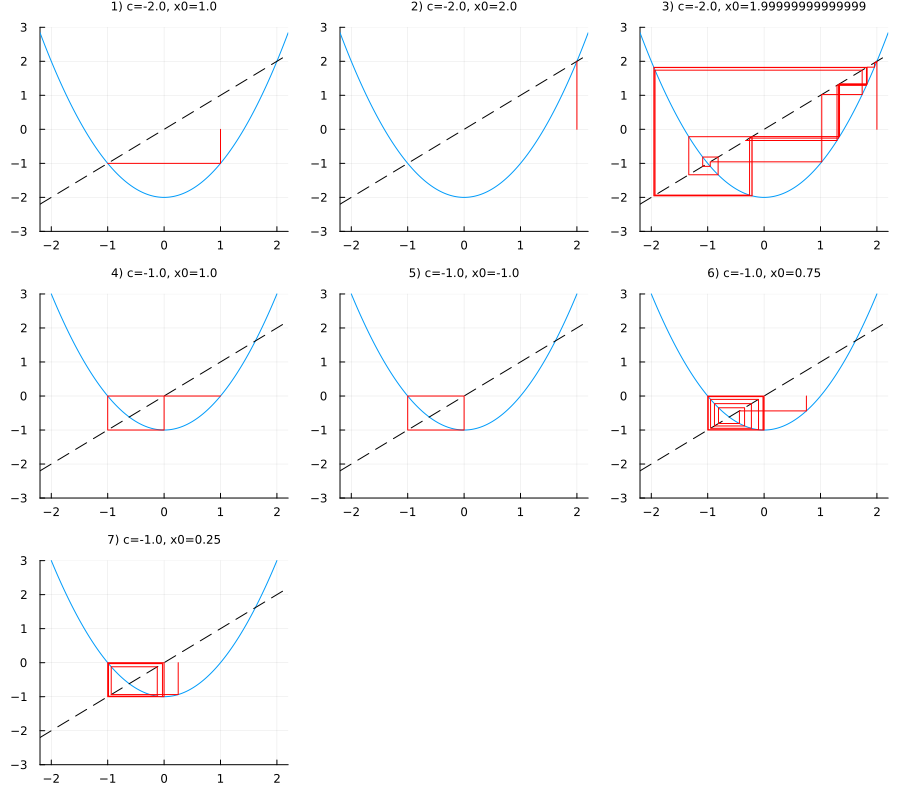
\includegraphics[width=.72\textwidth]{zad6_cobweb.png}
\caption{Iteracja graficzna dla przypadków 1--7 (czerwona linia); linia przerywana to $y = x$.}
\end{figure}

\subsection*{Interpretacja}
\begin{itemize}
    \item Dla $c = -2$ punkty stałe to $2$ i $-1$. Oba są odpychające ($|f'(2)| = 4$, $|f'(-1)| = 2$), ale w przypadkach 1 i 2 wszystkie obliczenia są dokładne, więc ciąg trafia w punkt stały i tam zostaje.
    \item W przypadku 3 odległość od $2$ wynosi $10^{-14}$ i rośnie ok. 4 razy na krok. Dla $n = 20$ mamy $1.989$, dla $n = 22$ już $1.827$, a potem ciąg skacze chaotycznie po $[-2, 2]$.
    \item To nie jest skutek zaokrągleń, tylko zachowanie samego odwzorowania. W \texttt{BigFloat} z tym samym $x_0$ ciąg przebiega tak samo (różnica $1.9 \cdot 10^{-7}$ dla $n = 30$ i $3.9 \cdot 10^{-4}$ dla $n = 40$). Zaokrąglenia też rosną, ale w 40 iteracjach nie zdążyły zmienić obrazu.
    \item Dla $c = -1$ punkty stałe $(1 \pm \sqrt{5})/2$ są odpychające ($|f'| \approx 3.24$ i $1.24$), ale istnieje cykl $0 \to -1 \to 0$, który przyciąga bardzo silnie, bo $f'(0) f'(-1) = 0$. Wszystkie przypadki 4--7 do niego dochodzą.
    \item Przypadki 4 i 5 są w cyklu już po 1--2 krokach. W przypadkach 6 i 7 ciąg dokładny tylko się do niego zbliża, ale w \texttt{Float64} trafia w $-1$ dokładnie: dla $n = 16$ i $n = 11$, bo odległość od $0$ jest wtedy tak mała, że $x_n^2 - 1$ zaokrągla się do $-1$.
\end{itemize}

\end{document}
